The objective of this work is to design and implement a Network-on-Chip (NoC) router for a $3 \times 3$ mesh system. The target mesh structure is illustrated in Figure~\ref{fig:mesh_3x3_pe}. The router is designed to support packet-based communication using fixed-width flits and deterministic XY routing, while also providing virtual-channel-based flow control.

\begin{figure}[htbp]
    \centering
    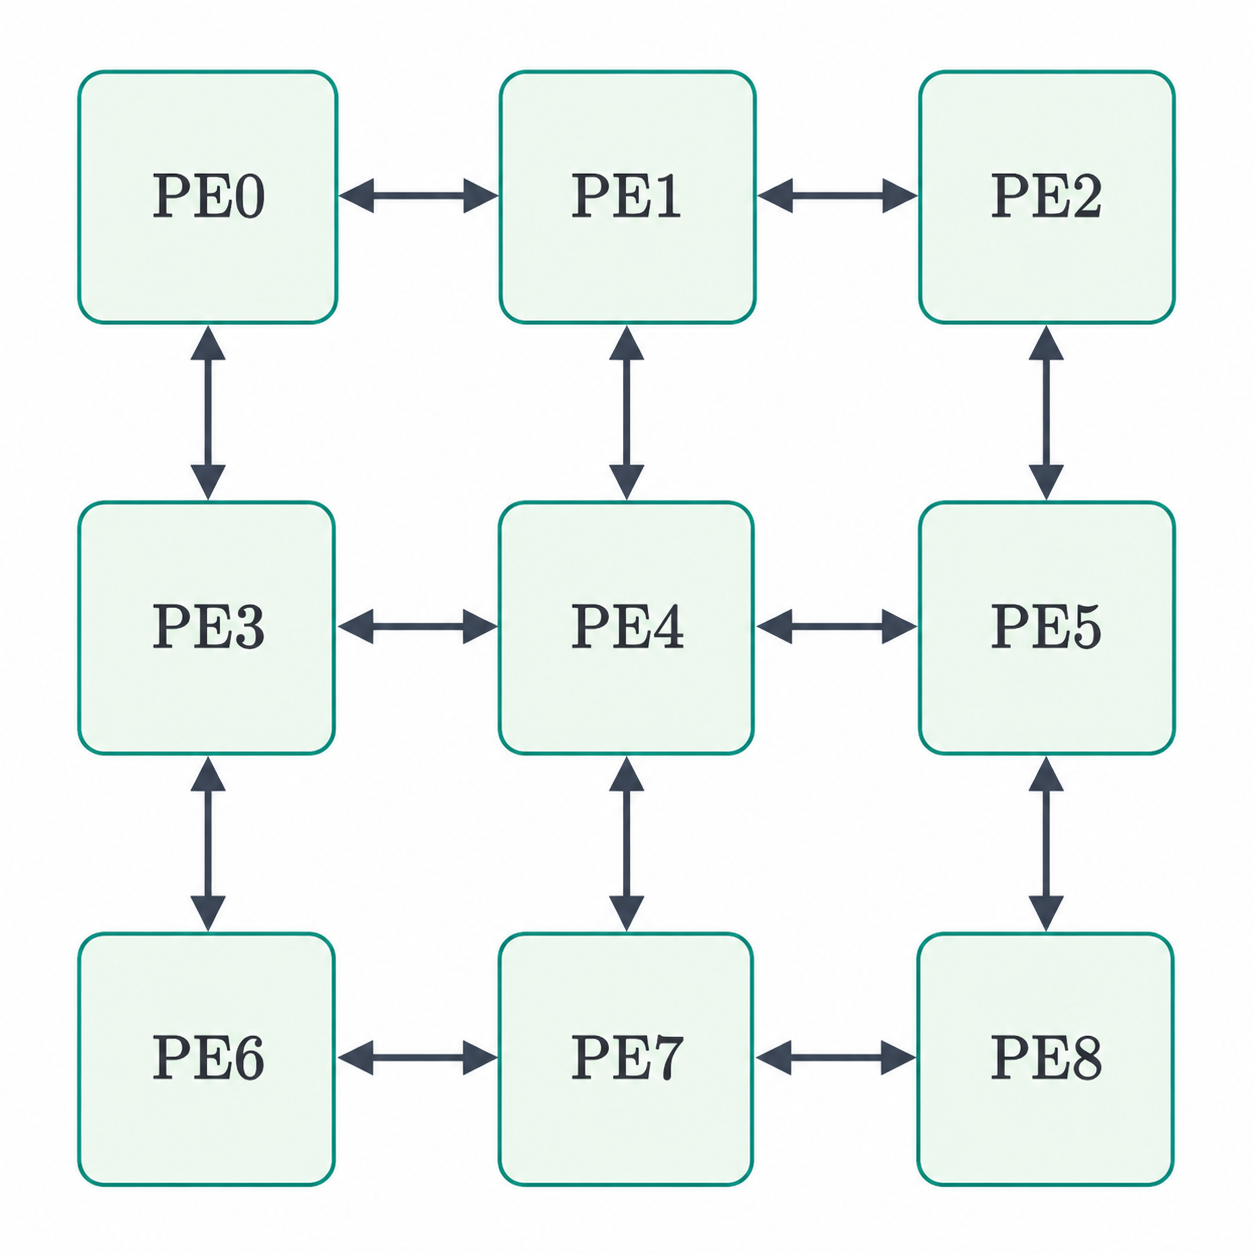
\includegraphics[width=0.4\textwidth]{images/ch3_design_and_implementation/3_times_3_mesh.png}
    \caption{$3 \times 3$ mesh structure}
    \label{fig:mesh_3x3_pe}
\end{figure}

The router first needs to provide the basic packet forwarding function. Each packet is sent from a source processing element to a destination processing element, and the routing decision is made according to the information carried in the header flit. Since a packet is divided into several flits, the router also has to make sure that flits belonging to the same packet follow the same reserved path and keep their original order. 

To organize the router operation, a three-stage pipeline is used. The first stage performs routing computation and virtual-channel allocation. The second stage is responsible for switch allocation, where the router decides which input can access the requested output port. The third stage performs switch traversal and sends the selected flit to the output side. By separating these functions into different stages, the design avoids putting too much logic into a single cycle and makes the implementation easier to meet timing.

Flow control is another important requirement in the router design. Since downstream buffers may become full, the router must be able to stop sending flits when the next router cannot accept more data. For this reason, the interface uses a valid-ready handshake together with credit-based flow control. A flit is transferred only when both valid and ready are asserted, while the returned credit information is used to indicate available buffer space in the downstream virtual channels.

Overall, the goal of this chapter is to present not only the implemented router structure, but also the design method used to connect routing decisions, virtual-channel allocation, flow control, and hardware implementation in a consistent router architecture.